\documentclass[aspectratio=169,11pt]{beamer}

\usepackage[T1]{fontenc}
\usepackage[utf8]{inputenc}
\usepackage{lmodern}
\usepackage{booktabs}
\usepackage{array}
\usepackage{amsmath}
\usepackage{graphicx}
\usepackage{tikz}
\usetikzlibrary{arrows.meta,positioning}

\definecolor{navy}{HTML}{1F3864}
\definecolor{blu}{HTML}{2A78D6}
\definecolor{ora}{HTML}{EB6834}

\usetheme{default}
\setbeamertemplate{navigation symbols}{}
\setbeamercolor{structure}{fg=navy}
\setbeamercolor{normal text}{fg=black!90}
\setbeamerfont{frametitle}{series=\bfseries,size=\large}
\setbeamertemplate{frametitle}{%
  \vspace{3pt}\begin{minipage}[b]{0.82\linewidth}\color{navy}\insertframetitle\end{minipage}%
  \hfill\raisebox{-1pt}{
\includegraphics[height=0.72cm]{figures/strathmore_logo_wide.png}}\par
  \vspace{-3pt}\color{navy}\rule{\linewidth}{0.6pt}}
\setbeamertemplate{footline}{%
  \hfill\color{black!50}\footnotesize Esther Muthui (223932) \hspace{1em} \insertframenumber\hspace{0.6cm}\vspace{5pt}}
\setbeamertemplate{itemize items}[circle]
\setbeamercolor{itemize item}{fg=navy}
\setbeamerfont{itemize/enumerate body}{size=\normalsize}
\setbeamerfont{itemize/enumerate subbody}{size=\small}
\setbeamersize{text margin left=0.9cm,text margin right=0.9cm}
\setbeamercolor{alerted text}{fg=ora!85!black}
\setbeamercolor{block title}{bg=navy,fg=white}
\setbeamercolor{block body}{bg=navy!7,fg=black}
\setbeamercolor{block title alerted}{bg=ora!85!black,fg=white}
\setbeamercolor{block body alerted}{bg=ora!10,fg=black}
\renewcommand{\arraystretch}{1.15}
\newcommand{\code}[1]{\texttt{#1}}
\newcommand{\hl}[1]{{\color{navy}\textbf{#1}}}

\begin{document}

% 1 title (10 seconds)
\begin{frame}[plain]
  \vspace{4pt}
  
\includegraphics[height=2.1cm]{figures/strathmore_logo.png}\par
  \vfill
  {\color{navy}\fontsize{30}{34}\selectfont\bfseries ThreatGuard ST-BMSE\par}
  \vspace{4pt}
  {\color{navy}\LARGE\bfseries County-level conflict escalation forecasting\par}
  \vspace{10pt}
  \rule{0.5\linewidth}{1pt}\par
  \vspace{8pt}
  {\large DSA 8401 Applied Machine Learning \textbullet{} Three-minute presentation\par}
  \vspace{3pt}
  {\large Esther Muthui (223932) \textbullet{} Strathmore University \textbullet{} November 2026\par}
  \vspace{3pt}
  {\large Lecturers: Prof. Javier Serrano and Emmanuel Bundi\par}
  \vspace{3pt}
  {\large Live service: \url{https://threatguard-stbmse.onrender.com}\par}
  \vfill
\end{frame}

% 2 problem and data (30 seconds)
\begin{frame}{The question, and the data}
  \begin{itemize}\setlength{\itemsep}{9pt}
    \item \hl{Question:} will a Kenyan county escalate into conflict \emph{next month}? A ranked, calibrated list tells an analyst where to look first.
    \item \hl{Data:} 47 counties $\times$ 120 months (2015--2024), 5{,}640 rows. The data are \alert{synthetic}, built to the proposal's design, so the results show how the method behaves, not what is true in Kenya.
    \item \hl{Fair test:} train up to 2019, tune on 2020--2021, report once on 2022--2024. Only information known at month $t$ is used to predict month $t{+}1$.
  \end{itemize}
\end{frame}

% 3 method (40 seconds)
\begin{frame}{Method: three learners, one blend, one threshold}
  \begin{itemize}\setlength{\itemsep}{7pt}
    \item Logistic regression, random forest and XGBoost, blended by a calibrated logistic stacker.
    \item Empirical-Bayes Markov features: how likely each county is to stay in or move into escalation, shrunk towards the overall rate.
    \item A missed escalation is worse than a false alarm, so the alert threshold minimises expected cost:
  \end{itemize}
  {\footnotesize
  \[
    \tau^\star=\arg\min_{\tau}\Big[\text{cost of a false negative}\times\text{false negatives}(\tau)+\text{cost of a false positive}\times\text{false positives}(\tau)\Big]
  \]
  \[
    \text{cost of a false negative}:\text{cost of a false positive}=5:1\;\;\text{(my assumption)}
  \]
  \par}
  {\footnotesize False negative: a real escalation with no alert. False positive: an alert with no escalation.\par}
\end{frame}

% 4 results (45 seconds)
\begin{frame}{Result: beats persistence, not a random forest}
  \centering
  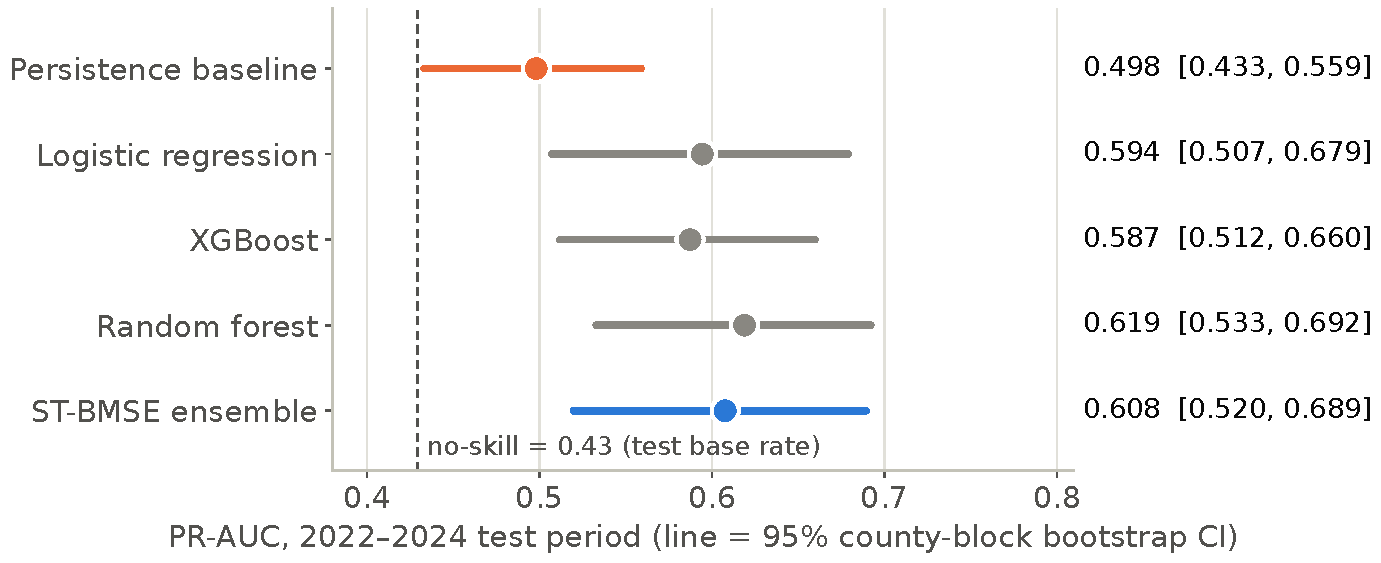
\includegraphics[width=0.78\linewidth]{figures/fig_results_s.pdf}
  \par\vspace{2pt}
  \begin{itemize}\setlength{\itemsep}{3pt}\small
    \item Precision-recall area under the curve on 2022--2024: \hl{0.61} against 0.50 for persistence, and the gain holds in all five rolling windows.
    \item Stacking does not beat a random forest (difference $-0.01$): the proposal's claim is not supported here.
  \end{itemize}
\end{frame}

% 5 system (35 seconds)
\begin{frame}{Delivered as a working system}
  \begin{columns}[T]
    \column{0.52\textwidth}
    \begin{itemize}\setlength{\itemsep}{6pt}\small
      \item One command rebuilds everything: ingest, features, train, evaluate.
      \item Quality gate on validation data only: a weak model is never saved or registered.
      \item MLflow tracking, Evidently drift report, 57 automated tests.
      \item FastAPI service in Docker; GitHub Actions builds, tests and publishes only what passes.
      \item Browser page: ranked counties, threshold slider, per-county detail.
    \end{itemize}
    \column{0.46\textwidth}
    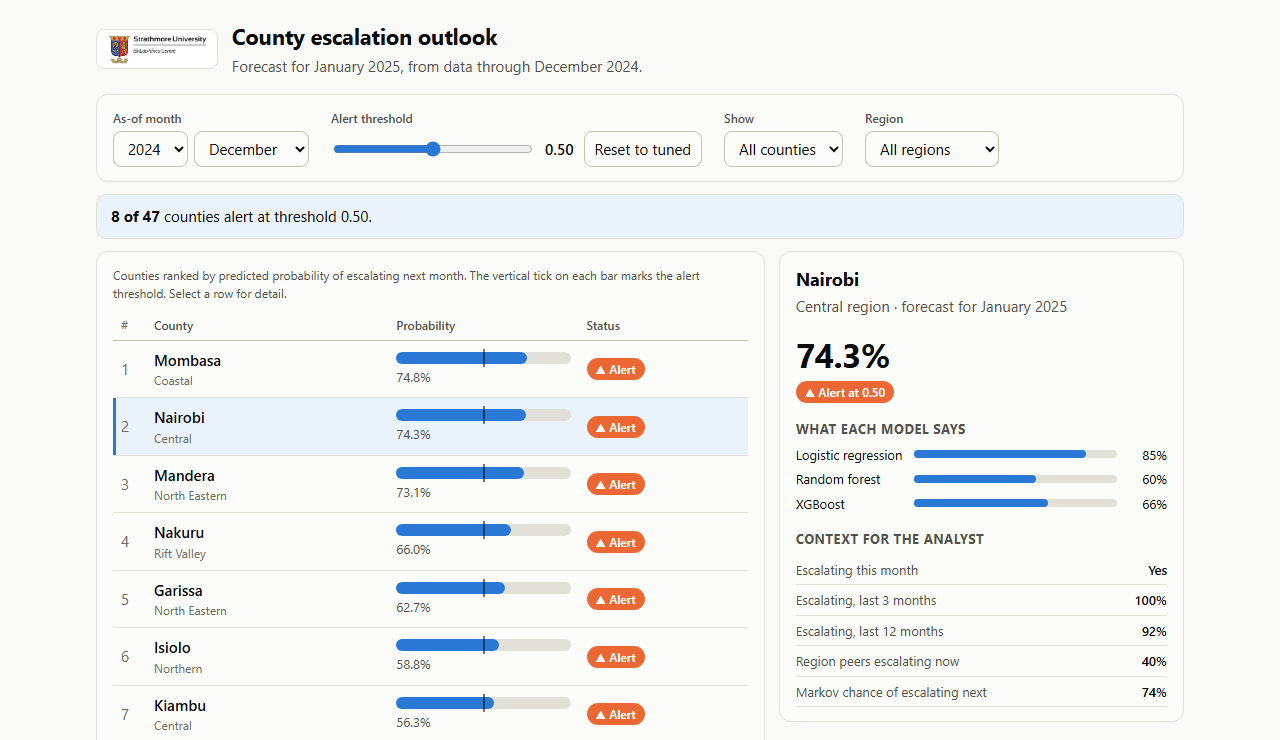
\includegraphics[width=\linewidth]{figures/ui_screenshot.png}
  \end{columns}
\end{frame}

% 6 limits and close (20 seconds)
\begin{frame}{Honest limits, and what comes next}
  \begin{columns}[T]
    \column{0.48\textwidth}
    \textbf{Limits}
    \begin{itemize}\setlength{\itemsep}{3pt}\small
      \item Synthetic data: no claim about real conflict.
      \item The 5:1 cost ratio is assumed, not elicited.
      \item The cost-tuned alert flags many counties (high false-alarm rate).
      \item The escalation rate rose from 20\% to 43\%, so the base rate drifts.
    \end{itemize}
    \column{0.48\textwidth}
    \textbf{Next}
    \begin{itemize}\setlength{\itemsep}{3pt}\small
      \item Real Armed Conflict Location and Event Data Project and Kenya National Bureau of Statistics data.
      \item Set the threshold with practitioners.
      \item Test a gated recurrent unit baseline.
    \end{itemize}
  \end{columns}
  \vfill
  \centering{\large\color{navy}\textbf{Thank you. Questions?}\par}
  \vspace{6pt}
\end{frame}

\end{document}
